\section{Introduction}

\begin{frame}{Adversarial Attacks}

\begin{enumerate}[$\Rightarrow$]
 \item Cause a machine learning model to make incorrect predictions.
  \item Achieved by perturbations that maximally degrade the information contained in an input signal.
  \pause
  \item Deep learning systems have been shown to be vulnerable to adversarial attacks
  \item Their outputs can be manipulated with imperceptibly small perturbations applied to the inputs
\end{enumerate}
\end{frame}

\begin{frame}{Adversarial Attacks}
\begin{figure}[H]
\centering
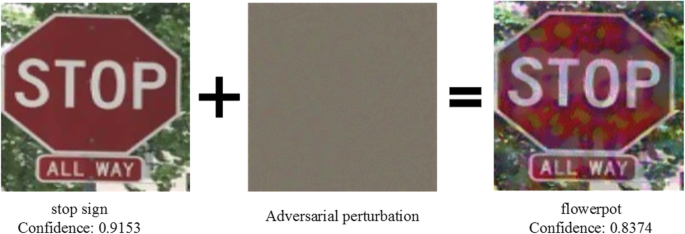
\includegraphics[width=0.8\columnwidth]{stop sign.png}
\end{figure}
\end{frame}

\begin{frame}{Optimal Adversarial Attacks}
% first paper
Some Notations:
\newline
U: the quantity (or label) of interest \newline
X: data generated from U \newline
\newline
Goal?\newline
Adding random perturbation E to X, producing random variable Y = X + E, such that the mutual information between U and Y = X + E is minimized
\pause 
\newline
\newline
NOTE: Since adding perturbations often introduces costs, we put constraints on the
perturbation E
\end{frame}

\begin{frame}{Optimal Adversarial Attacks}
the problem can be formulated as:
\begin{align*}
\min_{p(E|U,X)\in \mathcal{P}} I(U;X+E)
\end{align*}
where $\mathcal{P}$ is a set of admissible probability distributions.
\pause
\newline
for example, it can be:
\begin{align*}
\mathcal{P} &= \{p(E|U,X): \mathbb{E}[\norm{E}^2] \leq \epsilon, X \in \Omega\}
\end{align*}
\end{frame}

\begin{frame}{Robustness}
The property of a model to perform well and produce reliable results even when faced with unexpected or anomalous inputs
\newline 
\newline 
A robust loss (say, absolute error) may be preferred over a non-robust loss (say, squared error) due to its reduced sensitivity to large errors
\end{frame}

% TODO: connect robustness and regularization

\begin{frame}{Semi-Supervised Learning}
\begin{itemize}
    \item Labeling is hard, but there are often a lot of data
    \item Want to use unlabeled data to help training
\end{itemize}
\end{frame}

\begin{frame}{Regularization}
Adding a penalty term to the loss function \newline 
$\Rightarrow$  Discourages the model from having large weights for any of its features
\newline $\Rightarrow$ Prevent overfitting
\newline $\Rightarrow$ More robust to variations in the input data (Improve robustness)
\end{frame}

\begin{frame}{Regularization}
Can be interpreted as a prior distribution that reflects our educated a priori knowledge or belief regarding the model (from a Bayesian standpoint)
\pause 
\newline
\newline
A popular a priori belief $\rightarrow$ the outputs of systems are smooth with respect to spatial and/or temporal inputs
\end{frame}

%TOD


\section{Related Works}
\begin{frame}{Other Methods}
\begin{itemize}
  \item Label Propagation:
  \newline
  \newline
  Assign class labels to unlabeled training samples based on the belief that close input data points tend to have similar class labels
  \pause
  \newline
  \item Artificial Input:
  \newline
  \newline
Apply random perturbations to each input in order to generate artificial input points and encourage the model to assign similar outputs to the set of artificial inputs derived from the same point
\end{itemize}
\end{frame}
\begin{frame}{Other Methods}
\begin{enumerate}
  \item[?] But, what is the problem with these methods?
  \newline
  \newline
They often leave the predictor particularly vulnerable to a small perturbation in a specific direction called adversarial direction $\rightarrow$ it's the direction in the input
space in which the label probability $p(y = k|x)$ of the model
is most sensitive
\end{enumerate}
\end{frame}


\begin{frame}{Other Methods}
\begin{itemize}
\item  Contractive Loss:
\newline
\newline
Impose constraints on the Frobenius norm of the Jacobian matrix of the output with respect to the input
\newline 
\newline
 Deep Contractive Network, which imposes a layer-wise contraction penalty in a feed-forward neural network. The layer-wise penalty approximately minimizes the network outputs variance with respect to perturbations in the inputs, enabling the trained model to achieve “flatness” around the training data points.
\end{itemize}
\end{frame}

\begin{frame}{Other Methods}
\begin{enumerate}
  \item[?] But, what is the problem with this method?
  \newline
  \newline
  Computing the full Jacobian is computationally expensive and therefore they approximate it.
  \newline
  However, possibly because of their layer-wise approximation, their method was not successful in significantly decreasing the test error
%
\end{enumerate}
\end{frame}

\begin{frame}{Other Methods}
\begin{itemize}
\item  Generative adversarial networks (GANs)
\newline
\newline
Do not require an explicit definition of smoothness. 
\newline
\newline
Based on an objective function that trades off mutual information between observed examples and their predicted categorical class distribution, against the robustness of the classifier to an adversarial generative model. The resulting algorithm can be interpreted as a natural generalization of the generative adversarial networks (GAN) framework to robust classification against an optimal adversary.
\end{itemize}
\end{frame}

\begin{frame}{Other Methods}
\begin{enumerate}
  \item[?] But, what is the problem with this method?
  \newline
  \newline
In practice, these methods often require
careful tuning of many hyperparameters in the generative
model, and are usually not easy to implement without high
expertise in its optimization process.
\end{enumerate}
\end{frame}


\begin{frame}{Other Methods}
\begin{itemize}
  \item Adversarial Training:
  \newline 
  \newline
  Trains the model to assign to each input data a label that is similar to the labels to be assigned to its neighbors in the adversarial direction.
  \newline 
  Adversarial Direction $\rightarrow$ direction that can most greatly “deviate” the prediction of the model from the correct label.
\end{itemize}
\end{frame}

\begin{frame}{Other Methods}
\begin{enumerate}
  \item[?] But, what is the problem with this method?
  \newline
  \newline
Labeled data are needed for calculating the adversarial direction.
\end{enumerate}
\pause
\vspace{2em}
% \newline
% \hfill \break
% \hfill \break
Hence, the best method would be a method that considers Anisotropic smoothing and does not need labeled data to calculate the adversarial direction
\end{frame}

\section{Adversarial Training}
\begin{frame}{Some Notations}
I: Input dimension   \hfill  Q: Space of all labels
\newline
\newline
Input vector: $x\in R^{I}$ \hfill Output label: $y\in Q$
\newline
\newline
$p(y|x,\theta)$: Output distribution parameterized by $\theta$
\newline
\newline
$\hat{\theta}$: vector of the model parameters at a specific iteration step of the training process. 
\end{frame}

\begin{frame}{Some Notations}
Labeled Dataset: 
$\mathcal{D}_l = \{x_{l}^{n},y_{l}^{n}| n = 1,...,N_l\}$
\newline
\newline
Unlabeled Dataset:
$\mathcal{D}_{ul} = \{x_{ul}^{m}| m = 1,...,N_{ul}\}$
\end{frame}


\begin{frame}{Adversarial Training}
The loss function of adversarial training:
\\
\begin{align*}
L_{adv}(x_l, \theta) &= \D{q(y | x_l)}{p(y | x_l + r_{adv}, \theta)}\\
r_{adv} &= \argmax_{r; \norm{r} \le \epsilon} \D{q(y | x_l)}{p(y | x_l + r, \theta)}
\end{align*}
$D[p,p']$ :divergence between two distributions \(p\) and \(p'\)
\newline
$q(y|x_l)$ : true distribution of the output label, which is unknown.
\newline
\newline
Goal: approximate the true distribution by a parametric model $p(y|x_l,\theta)$ that is robust against adversarial attack to \(x\).
\end{frame}

\begin{frame}{Adversarial Training}
When the norm is $L_2$, adversarial perturbation can be approximated by:
\begin{align*}
r_{adv} &\approx \epsilon \frac{g}{\norm{g}_2}
\end{align*}
\begin{align*}
g = \nabla_{x_l} \D{h(y ; y_l)}{p(y | x_l, \theta)}\\
\end{align*}
\(g\) can be efficiently computed by backpropagation.
\newline
When the norm is $L_\infty$:
\begin{align*}
r_{adv} &\approx \epsilon \sign(g)
\end{align*}
\end{frame}

